\begin{figure}[H]
\centering
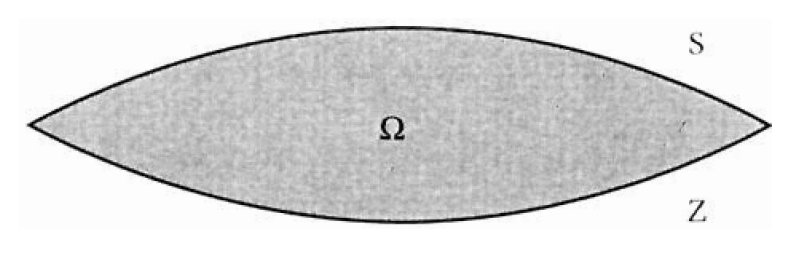
\includegraphics[width=.78\linewidth]{figures/lens-shaped-region-source.png}
\caption{一个透镜形区域}\label{fig:holmgren-lens-region}
\end{figure}

\subsection{Holmgren 唯一性定理}\label{sec:holmgren-uniqueness}

\PDEIndexMark{idx:holmgren-introduction}上一节的定理证明了非特征初值问题解的存在性与唯一性. 但唯一性仅在解析函数类中得到保证, 并未排除其他非解析解的存在. Holmgren 定理说明, 对线性方程, 这种情况不会发生; 这里只假定解足够光滑, 使偏微分方程中出现的所有导数都连续, 就证明唯一性 (利用本书后面定义的"广义"解概念, 还可以进一步放宽这一假设). 唯一性的证明通过证明一个"伴随"微分方程组解的存在性来实现. 为得到这一存在性, 使用 Cauchy-Kovalevskaya 定理, 因而需要假设方程的系数解析. 不过, 如果有一种不要求系数解析的存在性理论, 就不需要这一假设.

\subsubsection{主要思想概要}\label{subsec:holmgren-main-idea}

考虑线性方程组
\begin{equation}\label{eq:holmgren-linear-first-order-system}
a_{ij}^k(\bm{x})\dfrac{\partial u_j}{\partial x_k}+b_{ij}(\bm{x})u_j=0,\qquad i=1,\ldots,N.
\end{equation}
设 $\bm{u}=(u_1,\ldots,u_N)$ 是由两个曲面 $S$ 和 $Z$ 围成的"透镜形"区域 $\Omega\subset\mathbb{R}^n$ 内的解. 假设在 $Z$ 上 $\bm{u}=0$, 且 $S$ 非特征并解析. 还假设 \eqref{eq:holmgren-linear-first-order-system} 中的系数解析.

令 $v_i$, $i=1,\ldots,N$ 为 $C^1(\overline\Omega)$ 中的任意函数. 将 \eqref{eq:holmgren-linear-first-order-system} 的第 $i$ 个方程乘以 $v_i$, 对 $i$ 求和, 并在 $\Omega$ 上积分, 得到
\begin{equation}\label{eq:holmgren-integration-by-parts}
\begin{aligned}
0&=\int_\Omega v_i(\bm{x})a_{ij}^k(\bm{x})\dfrac{\partial u_j}{\partial x_k}(\bm{x})+
v_i(\bm{x})b_{ij}(\bm{x})u_j(\bm{x})\,\mathrm{d}\bm{x}\\
&=\int_\Omega-\dfrac{\partial}{\partial x_k}[v_i(\bm{x})a_{ij}^k(\bm{x})]u_j(\bm{x})
+v_i(\bm{x})b_{ij}(\bm{x})u_j(\bm{x})\,\mathrm{d}\bm{x}\\
&\quad+\int_{\partial\Omega}a_{ij}^k(\bm{x})v_i(\bm{x})u_j(\bm{x})n_k\,\mathrm{d}S,
\end{aligned}
\end{equation}
其中 $\bm{n}$ 为 $\partial\Omega$ 的外法向量.

现在假设 $\bm{v}$ 满足"伴随"偏微分方程组
\begin{equation}\label{eq:holmgren-adjoint-system}
-\dfrac{\partial}{\partial x_k}(a_{ij}^kv_i)+b_{ij}v_i=0,\qquad j=1,\ldots,N,
\end{equation}
及 $S$ 上的初始条件
\begin{equation}\label{eq:holmgren-adjoint-cauchy-data}
v_i=f_i
\end{equation}
则 \eqref{eq:holmgren-integration-by-parts} 化为
\begin{equation}\label{eq:holmgren-boundary-pairing}
0=\int_Sa_{ij}^k(\bm{x})f_i(\bm{x})u_j(\bm{x})n_k\,\mathrm{d}S.
\end{equation}


若这对 $S$ 上任意连续函数 $f_i$ 都成立, 就得到在 $S$ 上 $a_{ij}^ku_jn_k=0$; 又由于 $\det a_{ij}^kn_k\ne0$ ($S$ 非特征), 得到在 $S$ 上 $\bm{u}=0$.

Cauchy-Kovalevskaya 定理保证, 若 $f_i$ 解析, 则 \eqref{eq:holmgren-adjoint-system} 在 $S$ 的一个邻域内有解. 可惜, 一般不能断言这个邻域包含整个 $\Omega$. 如果它确实包含整个区域, 就能对解析的 $\bm{f}$ 得到 \eqref{eq:holmgren-boundary-pairing}. Weierstrass 逼近定理指出, $\mathbb{R}^n$ 的紧子集上的任意连续函数都可被多项式一致逼近. 因此, 若 \eqref{eq:holmgren-boundary-pairing} 对分量为多项式的 $\bm{f}$ 成立, 它也对连续的 $\bm{f}$ 成立.

\subsubsection{定理的陈述与证明}\label{subsec:holmgren-statement-proof}

为克服不能保证 \eqref{eq:holmgren-adjoint-system} 在整个 $\Omega$ 内有解这一困难, 将用单参数曲面族 $S_\lambda$ 替代曲面 $S$, 再沿 $\lambda$ 作"小步"推进. 更确切地说, 假定如下情形.

设 $D$ 为 $\mathbb{R}^n$ 中的有界区域, 且 \eqref{eq:holmgren-linear-first-order-system} 的系数在 $D$ 上解析. 令 $Z=D\cap\{x_n=0\}$, 并假设 $Z$ 非空且非特征. 设 $\Phi(\bm{x})$ 为定义在 $D$ 上的解析函数, 满足 $\nabla\Phi\ne0$, 并令 $S_\lambda=\{\Phi=\lambda\}\cap\{x_n\geq0\}$. 假设存在实数 $a$ 和 $b$, $a<b$, 使下列条件成立:

\begin{enumerate}
\item 集合 $\bigcup_{\lambda\in[a,b]}S_\lambda$ 是紧的.
\item $S_a$ 由位于 $Z$ 上的一个点构成.
\item 对 $a<\lambda<b$, $S_\lambda$ 为与 $Z$ 横截相交的正则曲面 (若两个曲面的法向量不共线, 就称其相交为横截相交). 此时 $S_\lambda$ 与 $Z$ 的交是一个正则 (解析) 的 $(n-2)$ 维曲面. 此外, 假设 $S_\lambda$ 非特征.
\end{enumerate}

\begin{figure}[H]
\centering
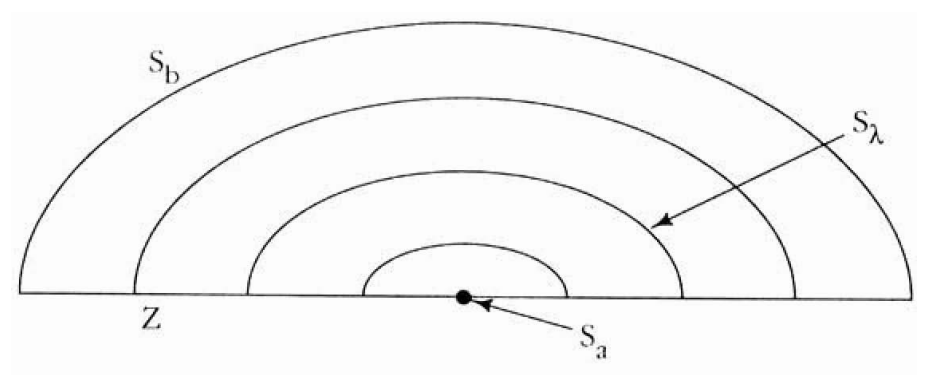
\includegraphics[width=.78\linewidth]{figures/holmgren-surface-family-source.png}
\caption{}\label{fig:holmgren-surface-family}
\end{figure}

将证明以下结果:

\begin{Theorem}
\label{thm:holmgren-uniqueness}
令 $\Omega=\{\bm{x}\in D\mid x_n>0,\ a<\Phi(\bm{x})<b\}$. 设 $\bm{u}\in C^1(\overline\Omega)$ 是 \eqref{eq:holmgren-linear-first-order-system} 的一个解, 且在 $\partial\Omega\cap\overline Z$ 上 $\bm{u}=0$. 那么在 $\overline\Omega$ 内 $\bm{u}=0$.
\end{Theorem}

\begin{Proof}令 $\Lambda=\{\lambda\in[a,b]\mid\bm{u}=0\text{ on }S_\lambda\}$. 已知 $a\in\Lambda$, 由 $\bm{u}$ 的连续性可得 $\Lambda$ 是闭的. 将证明 $\Lambda$ 在 $[a,b]$ 中也是开的. 由此得到 $\Lambda=[a,b]$, 从而定理成立.

注意, $\overline\Omega$ 是紧的, 因而存在不依赖于 $\bm{x}$ 的 $M,\rho$, 使每个 $\bm{x}\in\overline\Omega$ 都有 $a_{ij}^k$, $b_{ij}$ 和 $\Phi$ 属于 $C_{M,\rho}(\bm{x})$. 因此, 若在 $S_\mu$ 上指定 $C_{M,\rho}$ 类的 Cauchy 数据, 则 \eqref{eq:holmgren-adjoint-system} 的解存在于 $S_\mu$ 的一个 $\epsilon$ 邻域内, 其中 $\epsilon$ 不依赖于 $\mu\in(a,b]$. 注意, 任意多项式都属于某个 $C_{M,\rho}$, 其中可以将 $\rho$ 取得任意大, 代价是使 $M$ 也变大. 然而, \eqref{eq:holmgren-adjoint-system} 是线性的, 因而将 Cauchy 数据乘以常数因子, 并不改变解存在的区域. 所以, 使 \eqref{eq:holmgren-adjoint-system} 的解存在于 $S_\mu$ 的一个 $\epsilon$ 邻域内的 Cauchy 数据类包含所有多项式.

断言, 对给定的 $\lambda\in[a,b]$ 和 $\epsilon>0$, 存在 $\delta>0$, 使得只要 $\mu\in[a,b]$ 且 $|\mu-\lambda|<\delta$, $S_\lambda$ 就包含在 $S_\mu$ 的 $\epsilon$ 邻域内. 为此, 首先注意, 在任意点 $\bm{x}\in S_\lambda$ 的邻域内, 方程 $\Phi(\bm{x})=\mu$ 都可对某个坐标求解为 $x_i=x_i(x_1,\ldots,x_{i-1},x_{i+1},\ldots,x_n,\mu)$, 而若 $\bm{x}\in Z$ 且 $\lambda\ne a$, 则可选择 $i\ne n$. 若 $\lambda=a$, 则必须选择 $i=n$, 且 $x_n$ 是 $\mu$ 的递增函数. 在所有情形下, 一个直接结论是: 如果 $\delta(\bm{x})$ 取得充分小, 则对每个满足 $|\mu-\lambda|<\delta(\bm{x})$ 的 $\mu\in[a,b]$, 都存在点 $\bm{y}\in S_\mu$, 使 $|\bm{y}-\bm{x}|<\epsilon/2$. 由于 $S_\lambda$ 紧, 存在有限个点 $\bm{x}_k$, $k=1,\ldots,K$, 使以 $\bm{x}_k$ 为中心, 半径为 $\epsilon/2$ 的球覆盖 $S_\lambda$. 取 $\delta=\min\delta(\bm{x}_k)$ 即得断言.

现在假设 $\lambda\in\Lambda$, 且 $\mu\in(a,b]$ 满足 $|\mu-\lambda|<\delta$, 其中 $\delta$ 同上. 那么可以对 $S_\lambda$, $S_\mu$ 和 $Z$ 围成的区域应用上一节解释的论证. 从而得到在 $S_\mu$ 上 $\bm{u}=0$, 因此 $\mu\in\Lambda$.\end{Proof}

\begin{Example}
\label{ex:wave-cauchy-domain-of-determinacy}
考虑二维波动方程
\begin{equation}\label{eq:wave-determinacy-example}
u_{yy}-u_{xx}=0,
\end{equation}
在 $y=0$, $-1<x<1$ 上给定 Cauchy 数据. 令 $\Phi(x,y)=(x-y+1)(x+y-1)$, 并令 $D=(-1,1)\times(-1,1)$. 那么对 $-1\leq\lambda<0$, $S_\lambda$ 是双曲线 $(x-y+1)(x+y-1)=\lambda$ 位于顶点为 $(-1,0)$, $(1,0)$ 和 $(0,1)$ 的三角形内部的弧. 容易证明, 取 $a=-1$ 及任意 $b\in(-1,0)$, 定理的所有假设都满足. 由于各个 $S_\lambda$ 填满三角形内部, 给定的 Cauchy 数据确定了整个三角形内的 $u$. 一般地, 若 $Z$ 上的 Cauchy 数据确定了 $\Omega$ 内的 $u$, 则称 $\Omega$ 为 $Z$ 的一个\emph{决定域}.
\end{Example}

\subsubsection{Weierstrass 逼近定理}\label{subsec:weierstrass-approximation}

上述证明使用了以下定理, 称为 Weierstrass 逼近定理.

\begin{Theorem}
\label{thm:weierstrass-approximation}
设 $S$ 是 $\mathbb{R}^n$ 的紧子集, $f$ 是连续函数 $S\to\mathbb{R}$. 那么存在多项式序列 $p_m(\bm{x})$, 使 $p_m(\bm{x})\to f(\bm{x})$ 在 $S$ 上一致成立.
\end{Theorem}

\begin{Proof}取 $a_i$, $b_i$, $i=1,\ldots,n$, 使得 $S\subset P:=\prod_{i=1}^n(a_i,b_i)$. 由 Tietze-Urysohn 延拓定理, 可将 $f$ 延拓为整个 $\mathbb{R}^n$ 上的连续函数, 它在 $S$ 上与给定函数相同, 并在 $P$ 外为零. (大多数好的拓扑学教材都给出这一结果的证明.) 仍将延拓后的函数记为 $f$, 并证明 $f$ 可在 $P$ 上被多项式一致逼近. 不失一般性, 可假设 $0<a_i<b_i<1$.

先考虑一维情形, 即设 $f\in C(\mathbb{R})$, 且在区间 $(a,b)$ 外 $f=0$, 其中 $0<a<b<1$. 将构造多项式序列 $p_m$, 使 $p_m\to f$ 在 $[a,b]$ 上一致成立.

首先定义
\begin{equation}\label{eq:weierstrass-kernel-integrals}
I_m=\int_0^1(1-v^2)^m\,\mathrm{d}v,\qquad I_{m,\delta}=\int_\delta^1(1-v^2)^m\,\mathrm{d}v.
\end{equation}
从初等不等式
\begin{equation}\label{eq:weierstrass-kernel-integral-bounds}
I_m>\int_0^1(1-v)^m\,\mathrm{d}v=\dfrac1{m+1},\qquad I_{m,\delta}<(1-\delta^2)^m,
\end{equation}
得到对任意正的 $\delta$ 都有
\begin{equation}\label{eq:weierstrass-kernel-tail-limit}
\lim_{m\to\infty}\dfrac{I_{m,\delta}}{I_m}=0.
\end{equation}


现在选取 $\alpha$ 和 $\beta$, 使得 $0<\alpha<a<b<\beta<1$. 令
\begin{equation}\label{eq:weierstrass-one-dimensional-polynomial}
p_m(x)=\dfrac{\int_\alpha^\beta f(y)[1-(y-x)^2]^m\,\mathrm{d}y}{\int_{-1}^1(1-y^2)^m\,\mathrm{d}y}.
\end{equation}
显然, $p_m$ 是次数为 $2m$ 的多项式. 下面证明 $p_m$ 在 $[a,b]$ 上一致收敛到 $f$. 在分子中令 $y=v+x$, 得到
\begin{equation}\label{eq:weierstrass-three-integral-split}
\begin{aligned}
\int_{\alpha-x}^{\beta-x}f(v+x)(1-v^2)^m\,\mathrm{d}v
&=\int_{\alpha-x}^{-\delta}\cdots+\int_{-\delta}^{\delta}\cdots+\int_\delta^{\beta-x}\cdots\\
&=I_1+I_2+I_3.
\end{aligned}
\end{equation}


显然, $|I_1|$ 和 $|I_3|$ 都以 $MI_{m,\delta}$ 为界, 其中 $M$ 为 $|f|$ 的最大值. 现在给定 $\epsilon>0$, 选取 $\delta$, 使得当 $|v|\leq\delta$ 时有 $|f(v+x)-f(x)|\leq\epsilon$. 计算得到
\begin{equation}\label{eq:weierstrass-central-integral}
\begin{aligned}
I_2&=f(x)\int_{-\delta}^{\delta}(1-v^2)^m\,\mathrm{d}v\\
&\quad+\int_{-\delta}^{\delta}(f(x+v)-f(x))(1-v^2)^m\,\mathrm{d}v.
\end{aligned}
\end{equation}
右端第一项等于 $2f(x)(I_m-I_{m,\delta})$, 第二项可用 $2\epsilon I_m$ 估计. 合并所得估计, 得到
\begin{equation}\label{eq:weierstrass-uniform-error-estimate}
|p_m(x)-f(x)|\leq2M\dfrac{I_{m,\delta}}{I_m}+\epsilon.
\end{equation}


先将 $\epsilon$ 取得很小, 再相应地选取 $\delta$, 最后将 $m$ 取得充分大, 就可使这个量任意小.

在多维空间中, 类似地使用
\begin{equation}\label{eq:weierstrass-multivariable-polynomial}
p_m(\bm{x})=\dfrac{\int_{\alpha_1}^{\beta_1}\cdots\int_{\alpha_n}^{\beta_n}f(\bm{y})[1-(y_1-x_1)^2]^m\cdots[1-(y_n-x_n)^2]^m\,\mathrm{d}y_n\cdots\mathrm{d}y_1}{\left[\int_{-1}^1(1-\xi^2)^m\,\mathrm{d}\xi\right]^n}.
\end{equation}
\end{Proof}

\paragraph*{Problems}

\begin{enumerate}[label=\thesection.\arabic*.,ref=\thesection.\arabic*,start=18,series=book-problems]

\item\label{ex:laplace-cauchy-uniqueness} 设 $u$ 为 $\mathbb{R}^2$ 内 Laplace 方程的一个解, 并假设在 $y=0$ 且 $-1<x<1$ 时 $u=u_y=0$. 证明处处有 $u=0$.

\item\label{ex:wave-determinacy-boundary} 考虑在 $(-1,1)\times\{0\}$ 上给定 Cauchy 数据的波动方程 $u_{yy}-u_{xx}=0$. 证明任何决定域都不会延伸到顶点为 $(-1,0)$, $(0,1)$, $(1,0)$ 和 $(0,-1)$ 的正方形之外.

\item\label{ex:constant-coefficient-cauchy-uniqueness} 考虑一个常系数线性齐次一阶偏微分方程组, 使平面 $x_n=\mathrm{const.}$ 非特征. 证明, 任意在 $x_n=0$ 上为零的解都处处为零.

\item\label{ex:nonunique-zero-initial-heat-solution} 验证
\begin{equation}\label{eq:flat-in-time-heat-series}
u(x,t)=\sum_{m=0}^{\infty}\dfrac{x^{2m}}{(2m)!}\dfrac{\mathrm{d}^m}{\mathrm{d}t^m}\exp\left(\dfrac{-1}{t^2}\right)
\end{equation}
是 $u_t=u_{xx}$ 满足初始条件 $u(x,0)=0$ 的一个解. 为什么不能应用 Holmgren 定理? Hint: 用 Cauchy 公式估计 $\exp(-1/t^2)$ 的导数. 积分路径选取以 $t$ 为中心, 半径为 $t/2$ 的圆周.

\item\label{ex:polynomial-approximation-on-bounded-sets} 设 $f$ 是 $\mathbb{R}^n$ 上的连续函数. 证明, 存在多项式序列 $p_m$, 使 $p_m\to f$ 在整个 $\mathbb{R}^n$ 上成立, 并在任意有界集上一致成立. 举例说明, 一般而言, $p_m$ 不可能在整个 $\mathbb{R}^n$ 上一致收敛到 $f$.

\end{enumerate}
